\documentclass[12pt,a4paper,oneside]{erdc}
%\documentclass{erdc}
\usepackage[T1]{fontenc}		% Selecao de codigos de fonte.
\usepackage[utf8]{inputenc}		% Codificacao do documento (conversão automática dos acentos)
%\usepackage{lastpage}			% Usado pela Ficha catalográfica
\usepackage{indentfirst}		% Indenta o primeiro parágrafo de cada seção.
\usepackage{color}				% Controle das cores
\usepackage{graphicx}			% Inclusão de gráficos
%\usepackage{microtype} 			% para melhorias de justificação
\usepackage[brazil]{babel}
%\usepackage[brazilian,hyperpageref]{backref}	 % Paginas com as citações na bibl
%\usepackage[alf]{abntex2cite}	% Citações padrão ABNT
\usepackage{hyperref}
\usepackage{natbib}

\usepackage{lipsum}


\usepackage{Sweave}
\begin{document}
\Sconcordance{concordance:BP_Curso_TecComp_00_2019.tex:BP_Curso_TecComp_00_2019.Rnw:%
1 18 1 1 0 92 1 1 5 388 1}


\frontmatter

\laboratory{PPGE-UFPA}

\reportnum{BP/EcoS - Curso-DataScience-00-2019}

\program{Construção de Modelos e Indicadores Econômicos}

\title{Introdução ao Tratamento e Análise de Dados em R}

%\subtitle{Assessments and Report from Socioeconomic and Demographic Data in \\
%	      Small Cities in Amazon Delta}

\subtitle{ou Data Science para todos!}

\date{\today}

\author{S.~Rivero \and H.~Farias}

\affiliation{Programa de Pós-Graduação em Economia\\
  Instituto de Ciências Sociais Aplicadas\\
  Universidade Federal do Pará\\
  Rua Augusto Correia, 1\\
  Belém, Pará - 66.075-200}

\author{Equipe UFPA }


\affiliation{Faculdade de Economia \\
	Instituto de Ciências Sociais Aplicadas\\
	Universidade Federal do Pará\\
	Rua Augusto Correia, 1\\
	Belém, Pará - 66.075-200}


\coverart[width=\linewidth]{../figs/Capa}

\reporttype{Produto: Cursos}

\distribution{Propriedade BANPARÁ e PPGE-UFPA \\ (Distribuição Restrita)}

% \distribution{Distribution authorized to U.S. Government Agencies
% only; Test and Evaluation; November 2005.  Other requests should be
% referred to U.S. Army Engineer Research and Development Center}

%\additionalinfo{Supersedes ERDC/CREL AF-01-23}

\begin{abstract}
  \lipsum[12-13]
\end{abstract}

\disclaimer{
	
	This document is an output from the  Banpará Project 
	
	PPGE-UFPA report
	
	Distribution Restrictions
	
	\copyright 2019, All rights reserved
	
	\pagebreak
	
	}

\preparedfor{Banpará} 

\contractnum{FADESP-NO-CONTRATO}

\monitoredby{Banpará}

%\preparedfor{}




\maketitle

\tableofcontents


%\chapter*{Resumo Executivo}


\mainmatter

%%%%%%%%%%%%%%%%%%%%%%%%%%%%%%%%%%%%%%%%%%%%%%%%%
%  Chamadas de Bibliotecas e Variaveis Globais
%%%%%%%%%%%%%%%%%%%%%%%%%%%%%%%%%%%%%%%%%%%%%%%%%



\chapter*{Introdução}
\addcontentsline{toc}{section}{Introdução}

O R é uma suíte integrada de software que permite a recuperação, o tratamento, e a análise de dados\cite{Venables2011}. Pode se dizer que o R é um ambiente de tratamento de dados que permite ao usuário, além a análise de dados propriamente dita, escrever extensões e ampliar o seu escopo.

R é uma ferramenta de software livre que atende aos critérios da \textit{Free Software Foundation} e tem uma licença \textbf{GNU}\footnote{\url{https://www.gnu.org/}}

Algumas das funcionalidade do R são\cite{Venables2011}:
\begin{itemize}
	\item Ferramentas para manuseio e armazenamento de dados
	\item Um conjunto de operadores que permitem o cálculo numérico e a manipulação de matrizes
	\item Um enorme conjunto de bibliotecas para análise de dados
	\item Ferramentas para apresentação gráfica de dados e resultados
	\item Uma linguagem de programação orientada a objetos e extensível
	\item A possibilidade de estender a linguagem, suas bibliotecas e funções
\end{itemize}

\begin{figure}
	\centering
	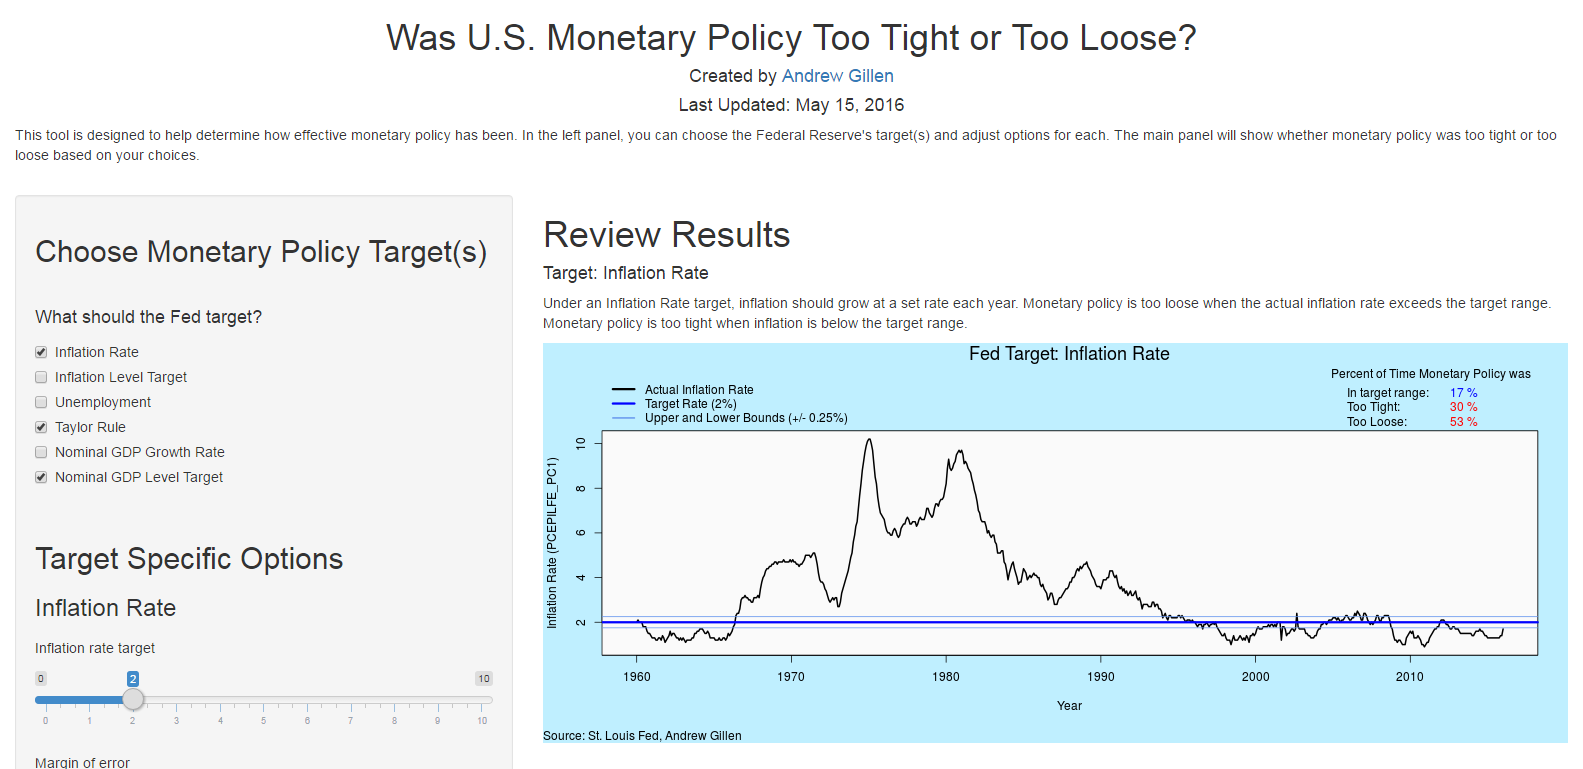
\includegraphics[width=\linewidth]{../figs/f-Intro-01-Monetary-Policy}
	\caption{Exemplo de \textit{Dashboard} de Política monetária usando R \cite{Showmeshiny2019}}
	\label{fig:f-intro-01}
\end{figure}

O R tem um conjunto extenso de ferramentas que permitem desde uma análise simples de regressão ou de aglomerados (\textit{cluster}) até apresentações de resultados extraídos de bancos de dados em larga escala com ferramentas de busca \textit{SQL}\footnote{Structured Query Language - \url{https://pt.wikipedia.org/wiki/SQL}} apresentas em páginas web\ref{fig:f-intro-01}.

Neste texto, iremos apresentar um conjunto de ferramentas de uso livre, a sua maioria de código aberto, que permitirão a extração, tratamento, análise e apresentação de dados, tanto para análises estatísticas mais diretas quanto para a tomada de decisões estratégicas de negócios.

%%%%%%%%%%%%%%%%%%%%%%%%%%%%%%%%%%%%%%%%%%%%%%%%%%%%%%%%%
%
%    CAPITULO
%
%%%%%%%%%%%%%%%%%%%%%%%%%%%%%%%%%%%%%%%%%%%%%%%%%%%%%%%%%

\chapter{Aula 1 - Instalando e Configurando o R e RStudio}

Nesta aula os alunos aprenderão a baixar o R e RStudio bem como aprenderão a utilizar bibliotecas em R


\section{Instalando o R e RStudio}

\subsection{Instalando o R}

Para instalar o R é preciso acessar o site \url{https://www.r-project.org/}. Os passos estão enumerados a seguir:

Nesta página clicar em \textbf{download R} que acessa a página - \url{https://cran.r-project.org/mirrors.html} - (Figura \ref{fig:f02-01})





\begin{figure}[htpb]
	\centering
	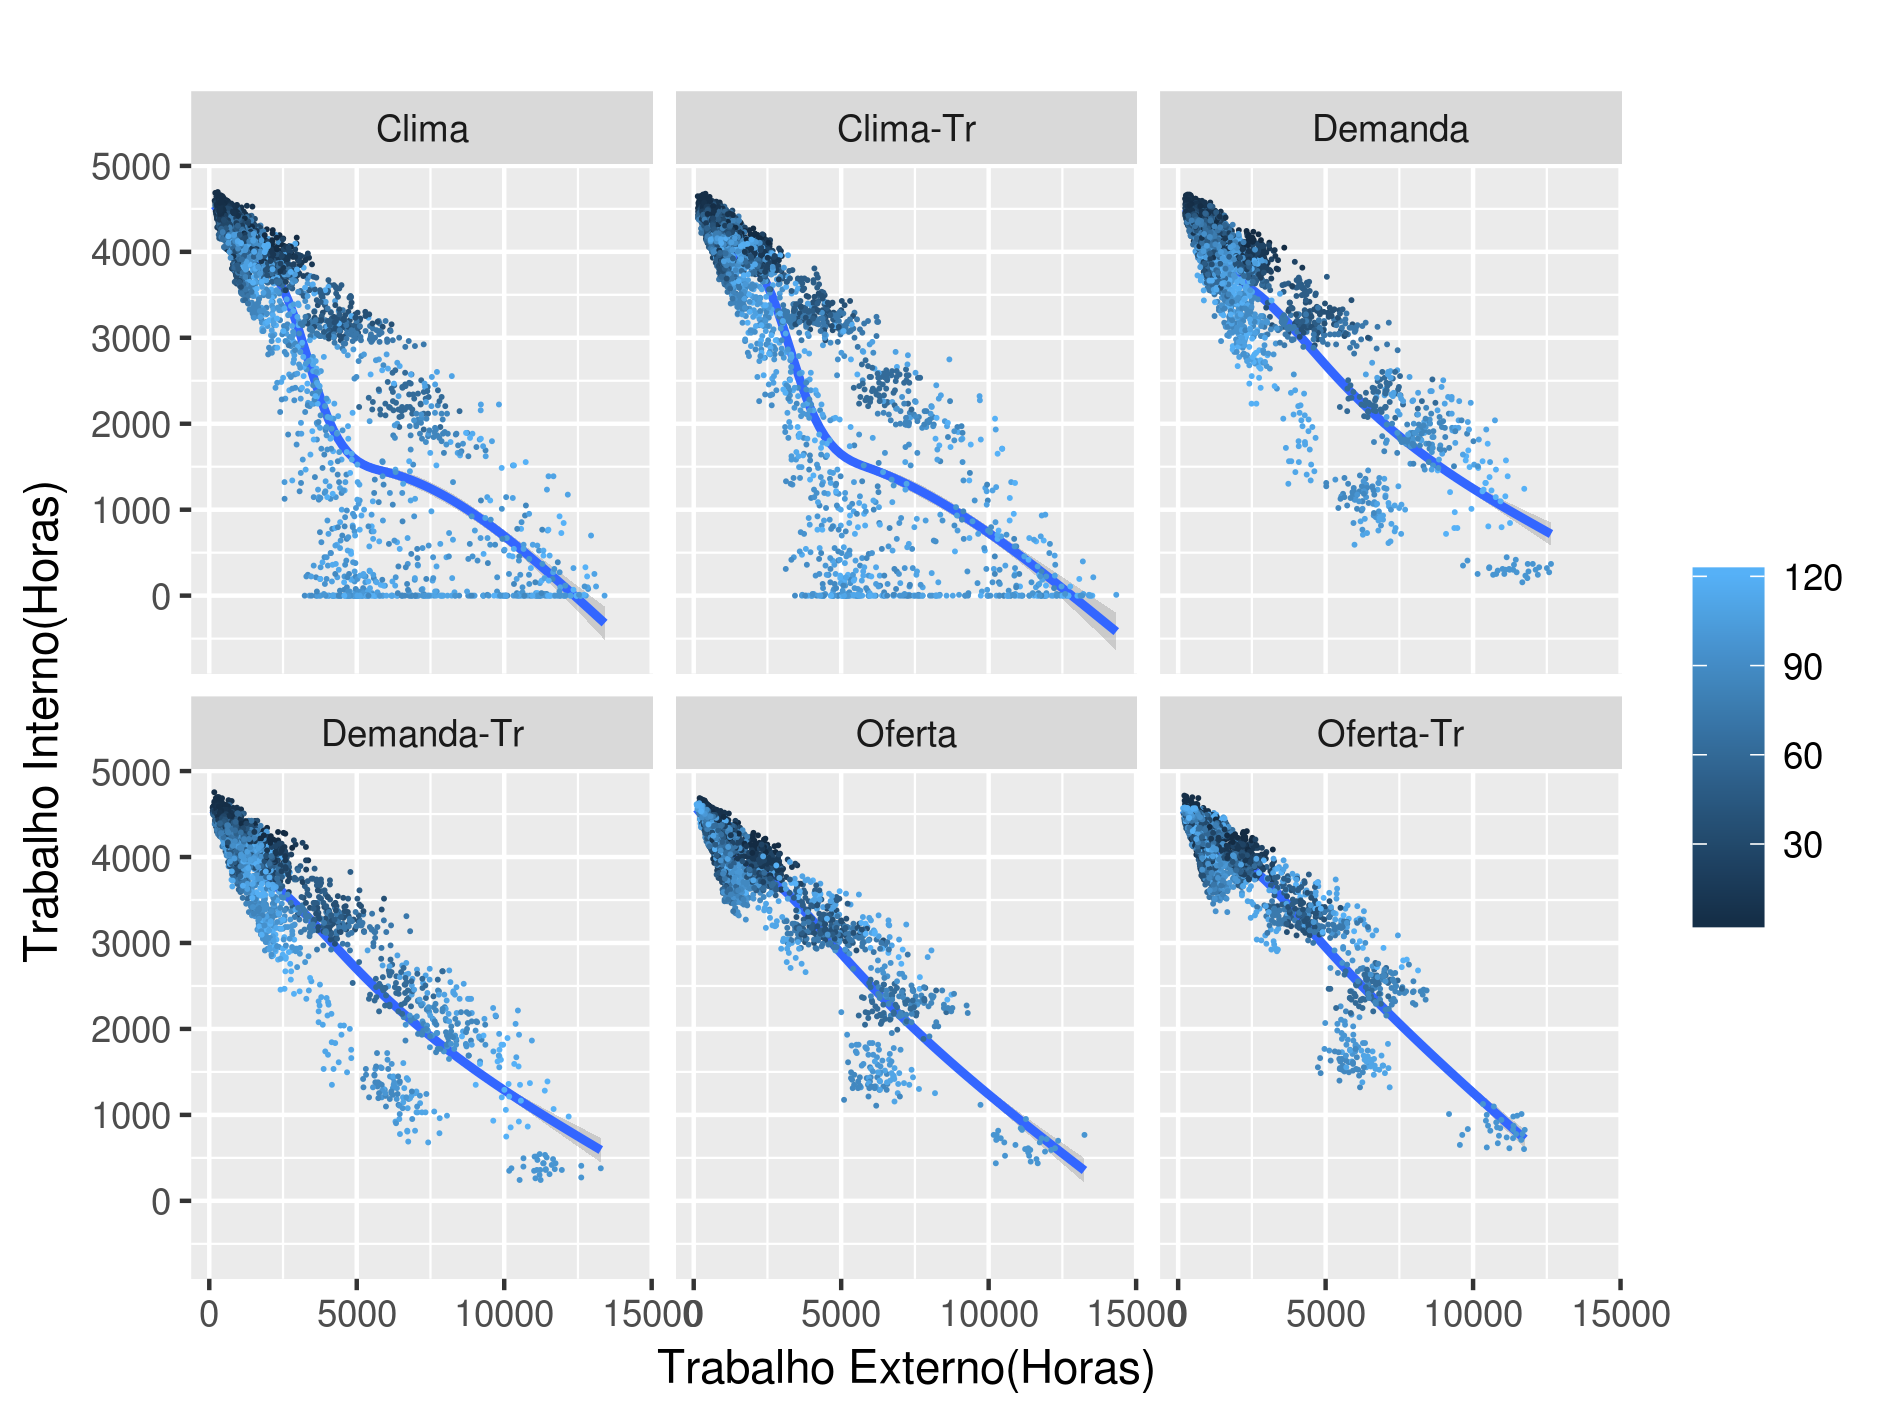
\includegraphics[width=\linewidth]{../figs/BP_Curso_TecComp_00_2019_f02-01}
	\caption{Nesta página clicar em \textbf{download R}}
	\label{fig:f02-01}
\end{figure}

Nesta página você seleciona o espelho que utilizará para baixar o R. Há sites no Brasil ou sítios em nuvem o item 0 - Cloud redirecionará automaticamente para sítios apoiados pelo Rstudio  -  \url{https://cloud.r-project.org/} (Figura \ref{fig:f02-02}) - A diferença entre os prefixos \textit{http} e \textit{https} é que os sites com \textbf{"s"} utilizam encriptação. Muitas vezes é necessário utilizar o \textit{https} em instalações cujos ambientes de TI exigem.



\begin{figure}[htpb]
	\centering
	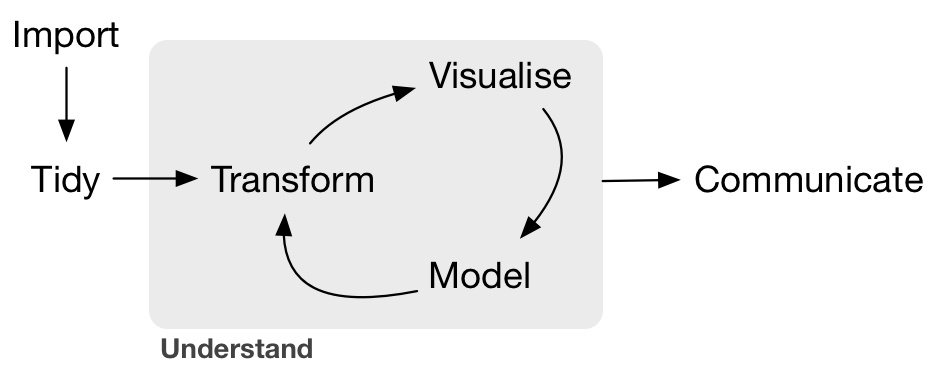
\includegraphics[width=\linewidth]{../figs/BP_Curso_TecComp_00_2019_f02-02}
	\caption{Aqui você seleciona o espelho que vai usar para baixar o R}
	\label{fig:f02-02}
\end{figure}

Você poderá baixar o R (por exemplo em \url{https://cloud.r-project.org/}) ou em algum dos outros espelhos citados anteriormente, de acordo com seu sistema operacional (Figura \ref{fig:f02-03}) Cada sistema (\textit{Linux}, \textit{MacOSX} ou \textit{Windows} tem uma rotina diferente para instalação. Aqui vamos explicar o sistema operacional mais comum (\textit{Windows}). Para outros sistemas, recomenda-se buscar instruções específicas em fóruns adequados.


\begin{figure}[htpb]
	\centering
	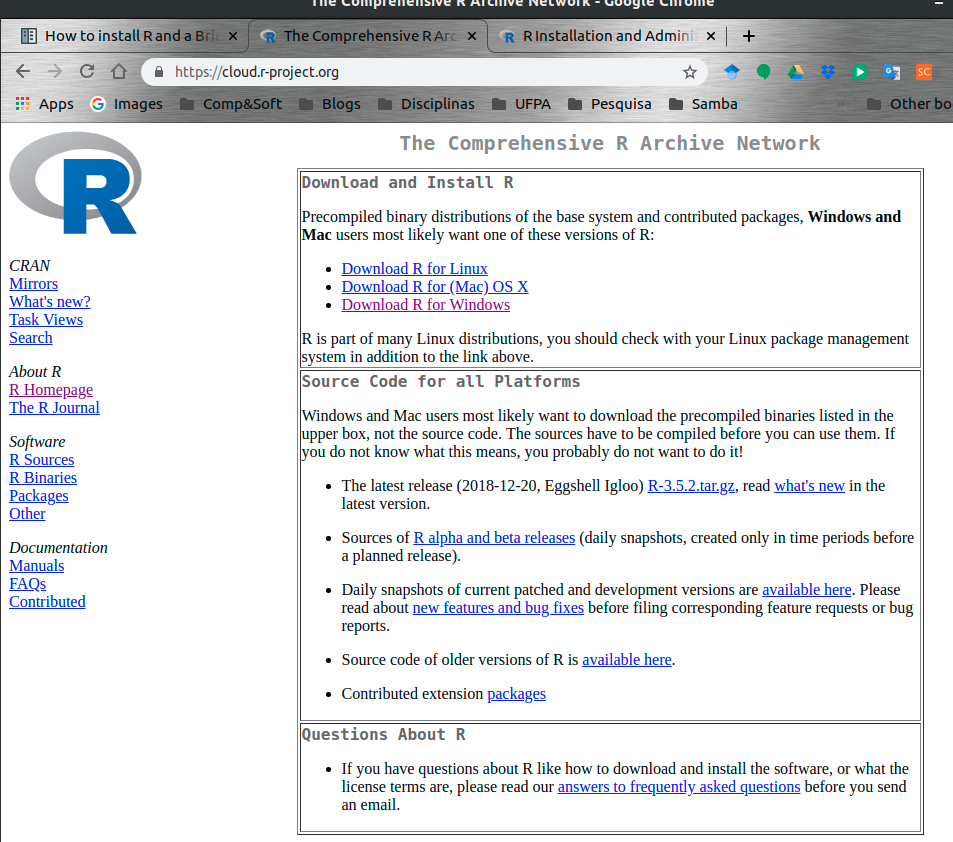
\includegraphics[width=\linewidth]{../figs/BP_Curso_TecComp_00_2019_f02-03}
	\caption{Sítio para baixar o R de acordo com seu sistema operacional}
	\label{fig:f02-03}
\end{figure}


Finalmente, para instalar o R, você pode executar o arquivo que está no link apresentado na Figura \ref{fig:f02-04}. Você baixará um arquivo \textbf{.exe} e, ao executá-lo, o instalador do \textit{Windows} tornará o programa disponível para uso na sua máquina. 

\begin{figure}[htpb]
	\centering
	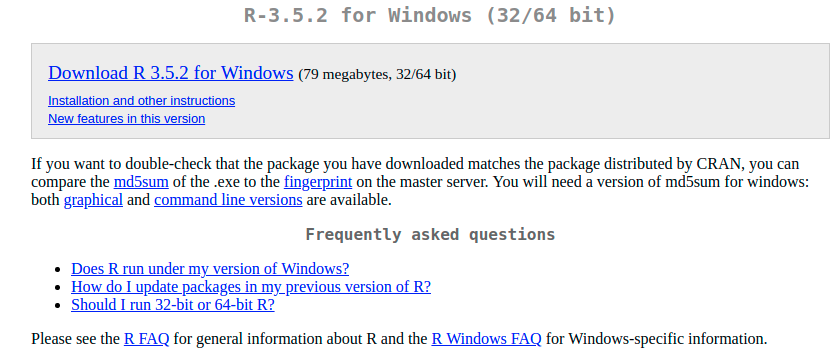
\includegraphics[width=\linewidth]{../figs/BP_Curso_TecComp_00_2019_f02-04}
	\caption{Página do Download do R}
	\label{fig:f02-04}
\end{figure}


Você pode conseguir mais informações sobre o R e os detalhes da instalação checando nos \textit{FAQs}\footnote{Frequently Asked Questions} dos sítios que você estiver acessando \url{https://cloud.r-project.org/bin/windows/base/rw-FAQ.html}, ou em \url{https://cran.r-project.org/doc/manuals/R-admin.html}



\subsection{Instalando o R Studio}

\url{https://www.rstudio.com/products/rstudio/}

\url{http://web.cs.ucla.edu/~gulzar/rstudio/}

\url{https://www.rstudio.com/products/rstudio/download/}

\url{http://rprogramming.net/download-and-install-rstudio/}


\section{Checando a Instalação Existente e os Requisitos}


\url{https://stackoverflow.com/questions/11103189/how-to-find-out-which-package-version-is-loaded-in-r}

\url{https://www.r-bloggers.com/list-of-user-installed-r-packages-and-their-versions/}

\url{https://community.rstudio.com/t/reinstalling-packages-on-new-version-of-r/7670}


\section{Pacotes no R}

\subsection{O conceito de pacote e para que serve}

\url{https://www.datacamp.com/community/tutorials/r-packages-guide}

\url{https://www.rstudio.com/products/rpackages/}

\url{http://r-pkgs.had.co.nz/}

\subsection{Como sei que pacotes eu preciso?}

\url{https://blog.revolutionanalytics.com/2017/01/cran-10000.html}

\url{https://cran.r-project.org/web/packages/available_packages_by_name.html}

\url{https://cran.r-project.org/web/packages/}

\subsection{Baixando os pacotes}

\url{https://www.r-bloggers.com/installing-r-packages/}

\url{https://www.r-bloggers.com/how-to-install-and-include-an-r-package/}

\url{http://kbroman.org/pkg_primer/pages/build.html}


\subsection{Resolvendo problemas de compilação}

\url{https://stackoverflow.com/questions/23135703/package-install-error-compilation-failed}

\url{https://support.rstudio.com/hc/en-us/community/posts/200522573-Can-t-install-packages}

\url{http://mazamascience.com/WorkingWithData/?p=1185}


\subsection{Utilizando os pacotes no seu programa R}

\url{https://www.statmethods.net/interface/packages.html}

\url{https://www.dummies.com/programming/r/how-to-install-load-and-unload-packages-in-r/}






%%%%%%%%%%%%%%%%%%%%%%%%%%%%%%%%%%%%%%%%%%%%%%%%%%%%%%%%%
%
%    CAPITULO
%
%%%%%%%%%%%%%%%%%%%%%%%%%%%%%%%%%%%%%%%%%%%%%%%%%%%%%%%%%
		
\chapter{Aula 2 - Acessando e Utilizando Bases de Dados}

Apresentar o conceito de Dataframe, os tipos de dados utilizados no R e os principais comandos  

\section{O ciclo de tratamento e análise de dados}

\section{Tipos de Dados em R}

\url{https://www.statmethods.net/input/datatypes.html}

\url{https://swcarpentry.github.io/r-novice-inflammation/13-supp-data-structures/}

\url{https://www.tutorialspoint.com/r/r_data_types.htm}

\url{http://www.r-tutor.com/r-introduction/basic-data-types}

\url{https://www.cyclismo.org/tutorial/R/types.html}

\url{https://stat.ethz.ch/R-manual/R-devel/library/base/html/typeof.html}

\section{Dataframes}

\url{https://www.tutorialspoint.com/r/r_data_frames.htm}

\url{https://www.datamentor.io/r-programming/data-frame/}

\url{http://www.r-tutor.com/r-introduction/data-frame}

\url{https://stat.ethz.ch/R-manual/R-devel/library/base/html/data.frame.html}

\url{https://www.tutorialgateway.org/data-frame-in-r/}

\url{https://datacarpentry.org/R-ecology-lesson/02-starting-with-data.html}

\url{https://www.statmethods.net/input/importingdata.html}

\section{Acessando Arquivos no computador}

\url{https://www.datacamp.com/community/tutorials/r-data-import-tutorial?utm_source=adwords_ppc&utm_campaignid=1455363063&utm_adgroupid=65083631748&utm_device=c&utm_keyword=&utm_matchtype=b&utm_network=g&utm_adpostion=1t1&utm_creative=332602034364&utm_targetid=dsa-473406573035&utm_loc_interest_ms=&utm_loc_physical_ms=1001610&gclid=Cj0KCQiA5NPjBRDDARIsAM9X1GLkgYWekNMkjHQnsTnRAzV7_gVEiwAqyW9CPisvAqFv2mNXzwarSlIaAgdZEALw_wcB}

\url{http://rprogramming.net/read-csv-in-r/}

\url{https://www.rdocumentation.org/packages/gdata/versions/2.18.0/topics/read.xls}

\url{https://stat.ethz.ch/R-manual/R-devel/library/utils/html/read.fwf.html}

\url{https://riptutorial.com/r/example/31447/importing-fixed-width-files}


\section{Acessando Bases de dados via \textit{APIs}}

\url{https://www.r-bloggers.com/accessing-apis-from-r-and-a-little-r-programming/}

\url{https://cran.r-project.org/web/packages/httr/vignettes/api-packages.html}

\url{https://zapier.com/learn/apis/}

\url{https://www.earthdatascience.org/courses/earth-analytics/get-data-using-apis/API-data-access-r/}



\section{Trabalhando com bases de dados muito grandes}

\url{http://dept.stat.lsa.umich.edu/~jerrick/courses/stat701/notes/sql.html}

\url{https://datacarpentry.org/R-ecology-lesson/05-r-and-databases.html}

\url{https://db.rstudio.com/}

\url{http://www.columbia.edu/~sjm2186/EPIC_R/EPIC_R_BigData.pdf}

\url{https://www.rstudio.com/resources/webinars/working-with-big-data-in-r/}

\url{https://rpubs.com/msundar/large_data_analysis}






%%%%%%%%%%%%%%%%%%%%%%%%%%%%%%%%%%%%%%%%%%%%%%%%%%%%%%%%%
%
%    CAPITULO
%
%%%%%%%%%%%%%%%%%%%%%%%%%%%%%%%%%%%%%%%%%%%%%%%%%%%%%%%%%

\chapter{Aula 3 - Limpando e organizando seus dados}

	\section{O que é uma boa base de dados e que tipos de bases existem?}
	
	\section{dplyr}
	
	\section{tidyr}
	
	\section{tidyverse}






%%%%%%%%%%%%%%%%%%%%%%%%%%%%%%%%%%%%%%%%%%%%%%%%%%%%%%%%%
%
%    CAPITULO
%
%%%%%%%%%%%%%%%%%%%%%%%%%%%%%%%%%%%%%%%%%%%%%%%%%%%%%%%%%

\chapter{Aula 4 - Apresentando Resultados}

	\section{Rmarkdown - Preparando o relatório enquanto você analisa os dados}
	
	\section{Gerando dados sintetizados - Utilizando dataframes}
	
	\section{Gerando Tabelas}
	
		\subsection{xtable}
		
		\subsection{stargazer}





%%%%%%%%%%%%%%%%%%%%%%%%%%%%%%%%%%%%%%%%%%%%%%%%%%%%%%%%%
%
%    CAPITULO
%
%%%%%%%%%%%%%%%%%%%%%%%%%%%%%%%%%%%%%%%%%%%%%%%%%%%%%%%%%


\chapter{Aula 5 - Gerando estatísticas dos Dados}

	\section{Estatísticas Descritivas}
	
	\section{Correlação}
	
	\section{Apresentando os Resultados em Gráficos}
	
		\subsection{Gráficos Simples}
		
		\subsection{Bibliotecas de Gráficos}






%%%%%%%%%%%%%%%%%%%%%%%%%%%%%%%%%%%%%%%%%%%%%%%%%%%%%%%%%
%
%    CAPITULO
%
%%%%%%%%%%%%%%%%%%%%%%%%%%%%%%%%%%%%%%%%%%%%%%%%%%%%%%%%%

\chapter{Aula 6 - Apresentando Resultados}

	\section{ggplot}

	\section{shiny}




%%%%%%%%%%%%%%%%%%%%%%%%%%%%%%%%%%%%%%%%%%%%%%%%%%%%%%%%%
%
%    CAPITULO
%
%%%%%%%%%%%%%%%%%%%%%%%%%%%%%%%%%%%%%%%%%%%%%%%%%%%%%%%%%

\chapter{Aula 7 - Utilizando modelos}

	\section{Regressão}
	
		\subsection{Executando a Regressão}
		
		\subsection{Apresentando os resultados da Regressão}
	
	\section{Gerando Dashboards}



%%%%%%%%%%%%%%%%%%%%%%%%%%%%%%%%%%%%%%%%%%%%%%%%%%%%%%%%%
%
%    CAPITULO
%
%%%%%%%%%%%%%%%%%%%%%%%%%%%%%%%%%%%%%%%%%%%%%%%%%%%%%%%%%
%
\chapter{Aula 8 - Encerramento do Curso}




\chapter{Onde aprender mais?}
\addcontentsline{toc}{section}{Onde aprender mais?}



%\bibliographystyle{unsrt}
\bibliographystyle{alpha}
\bibliography{../bib/bibliografia}

%\appendix

%\chapter{Tabelas demográficas}

%\lipsum[12-16]

%\begin{equation}
%  \label{eq:C}
%  \frac{\partial H}{\partial x} = -X
%\end{equation}

%\chapter{PeCiDAm}

%\lipsum[16-22]




\end{document}
